\chapter{Introduction}
Aim of this project is to carry out a comparative analysis at system level between different typology of CMOS multiplexers. We will perform several evaluations concerning the static and dynamic power consumption, the occupied area and time delay in different digital circuit configurations, within 2010 HP, LOP and LSTP technologies. Physical constants, system parameters and technological variables have been taken from TAMTAMS, a useful tool allowing to predict system level features starting from technology variables. In this project we will present multiplexer circuits built with NAND gates, enabling a fast and interesting analysis of the performances.

\section{Multiplexer architecture}
The multiplexer (\ref{mux_blocchi}) is a combinational logic circuit designed to switch several input lines toward a single common output line by the application of a control signal.\\
\begin{figure}[!h]
	\centering
	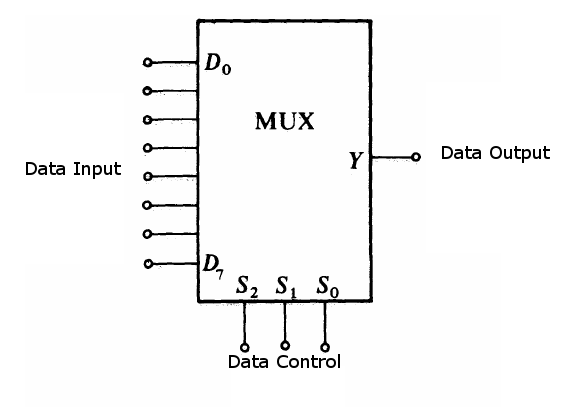
\includegraphics[scale=0.5]{immagini/mux_blocchi.png}
	\caption{\textit{Multiplexer block diagram.}} 
	\label{mux_blocchi}
\end{figure}
\newline
Multiplexers can be either digital circuits made from high speed logic gates used to switch digital or binary data.
In digital electronics, multiplexers are also known as data selectors because they can “select” among different input lines.
They are used as a method to reduce number of data lines required in a circuit design or when a single data line or data bus is used to transfer two or more different digital signals.\\
Generally, the selection of each input line in a multiplexer is controlled by an additional set of inputs called control lines, and according to the binary condition of these control inputs, either “high” or “low”, the appropriate data input is connected directly to the output.\\
Normally, a multiplexer has an even number of ($2^N$) data input lines with $N$ selection inputs.\\
In figure \ref{mux_funz} is shown the logic circuit of the simplest multiplexer unit next to his truth table. When the selection input is \textit{S = 0}, the upper AND gate is selected (\textit{G0}) and the digital data (0 or 1) present at the input data \textit{D0} is transferred to the output. Conversely when \textit{S = 1}, the upper AND gate is enabled (\textit{G1}) and the value \textit{D1} it is transferred at the output. The logic function that expresses the output is
\begin{equation}
Y=D_0\bar S+D_1S.
\label{eq1}
\end{equation}
\begin{figure}[!h]
	\centering
	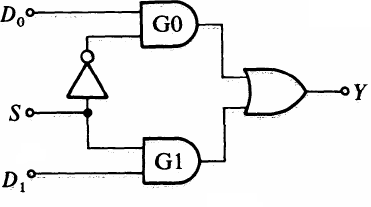
\includegraphics[scale=0.6]{immagini/mux_1.png}
	\caption{\textit{Logic circuit implementation of a multiplexer with two inputs.}} 
	\label{mux_1}
\end{figure}

\begin{figure}[!h]
	\centering
	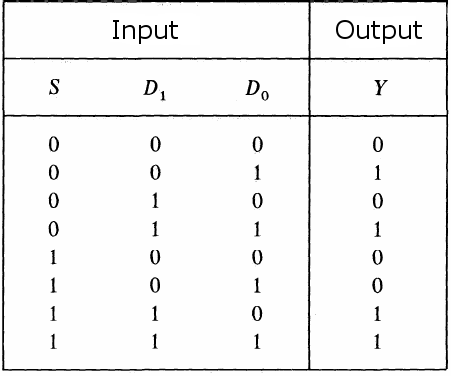
\includegraphics[scale=0.4]{immagini/mux_fun1.png}
	\caption{\textit{Truth table.}} 
	\label{mux_funz}
\end{figure}
\newpage
\section{Multiplexer with NAND gates}
In principle, any combinatorial logic function can be realized with enough NAND gates through the two De Morgan theorems:
\begin{equation}
\overline{A\cdot B}= \overline{A} + \overline{B}
\label{de1}
\end{equation}
\begin{equation}
\overline{A + B}= \overline{A} \cdot \overline{B}
\label{de2}
\end{equation}
The first \ref{de1} one mentions that the negated product of two variables is equal to the sum of negated variables.\\
The second \ref{de2} theorem is stating that the negated sum of two variables is equal to the product of the single negated variables.\\
Applying to the figure \ref{mux_1} the De Morgan's theorems allows to redefine the entire circuit using only NAND gates.
\begin{equation}
Y=\overline{\overline{D_0 + \overline{S + S}}+\overline{D_1+S}}
\label{de3}
\end{equation}
\begin{figure}[!h]
	\centering
	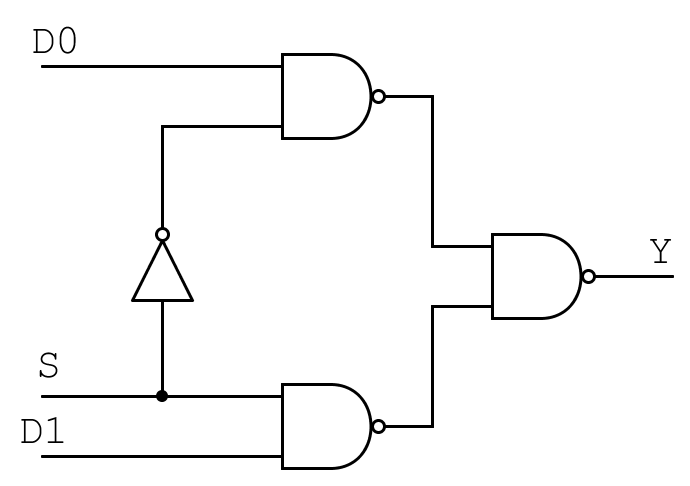
\includegraphics[scale=0.5]{immagini/mux_3.png}
	\caption{\textit{Circuit implementation of a multiplexer with two inputs optimized.}} 
	\label{mux_2}
\end{figure}
\newline
The inverter can be easily imagined as a NAND port with the inputs connected together.
\begin{figure}[!h]
	\centering
	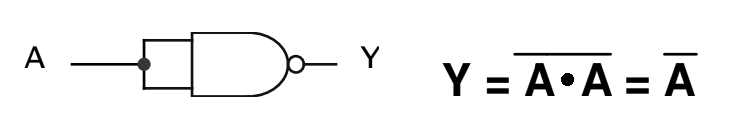
\includegraphics[scale=0.6]{immagini/not_nand.png}
	\caption{\textit{Inverter made with a NAND}} 
	\label{not}
\end{figure}
\newline
By implementing these properties the logical scheme becomes:
\begin{figure}[!h]
	\centering
	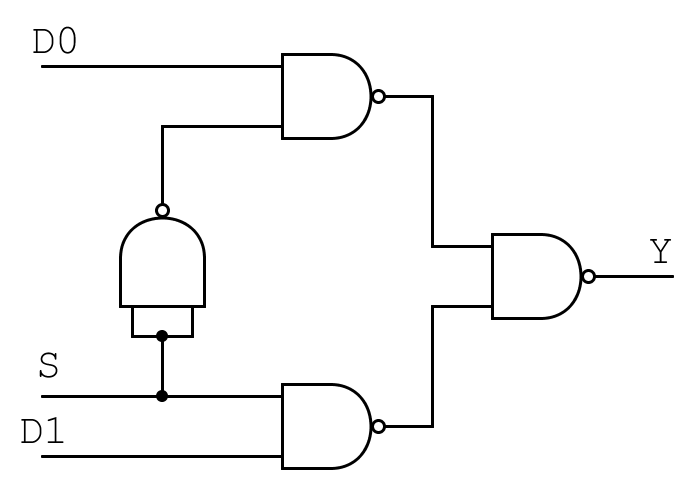
\includegraphics[scale=0.4]{immagini/2_to_1_1bit}
	\caption{\textit{Circuit implementation of a  multiplexer 2 to 1 with only NAND gates.}} 
	\label{2_to_1_1bit}
\end{figure}
We choose to use basic NAND configurations as they allow a simpler approach, namely to evaluate the area and power consumption of a single NAND gate and multiply it by the number of those that make up the circuit.\\ With a single 2 to 1 mux unit is possible to build more complex multiplexers, showing a tree circuit structure. In figure \ref{8_to_1_1bit} is reported a multiplexer 8 to 1  with a word of 1 bit, using 24 NAND gates.
\begin{figure}[!h]
	\centering
	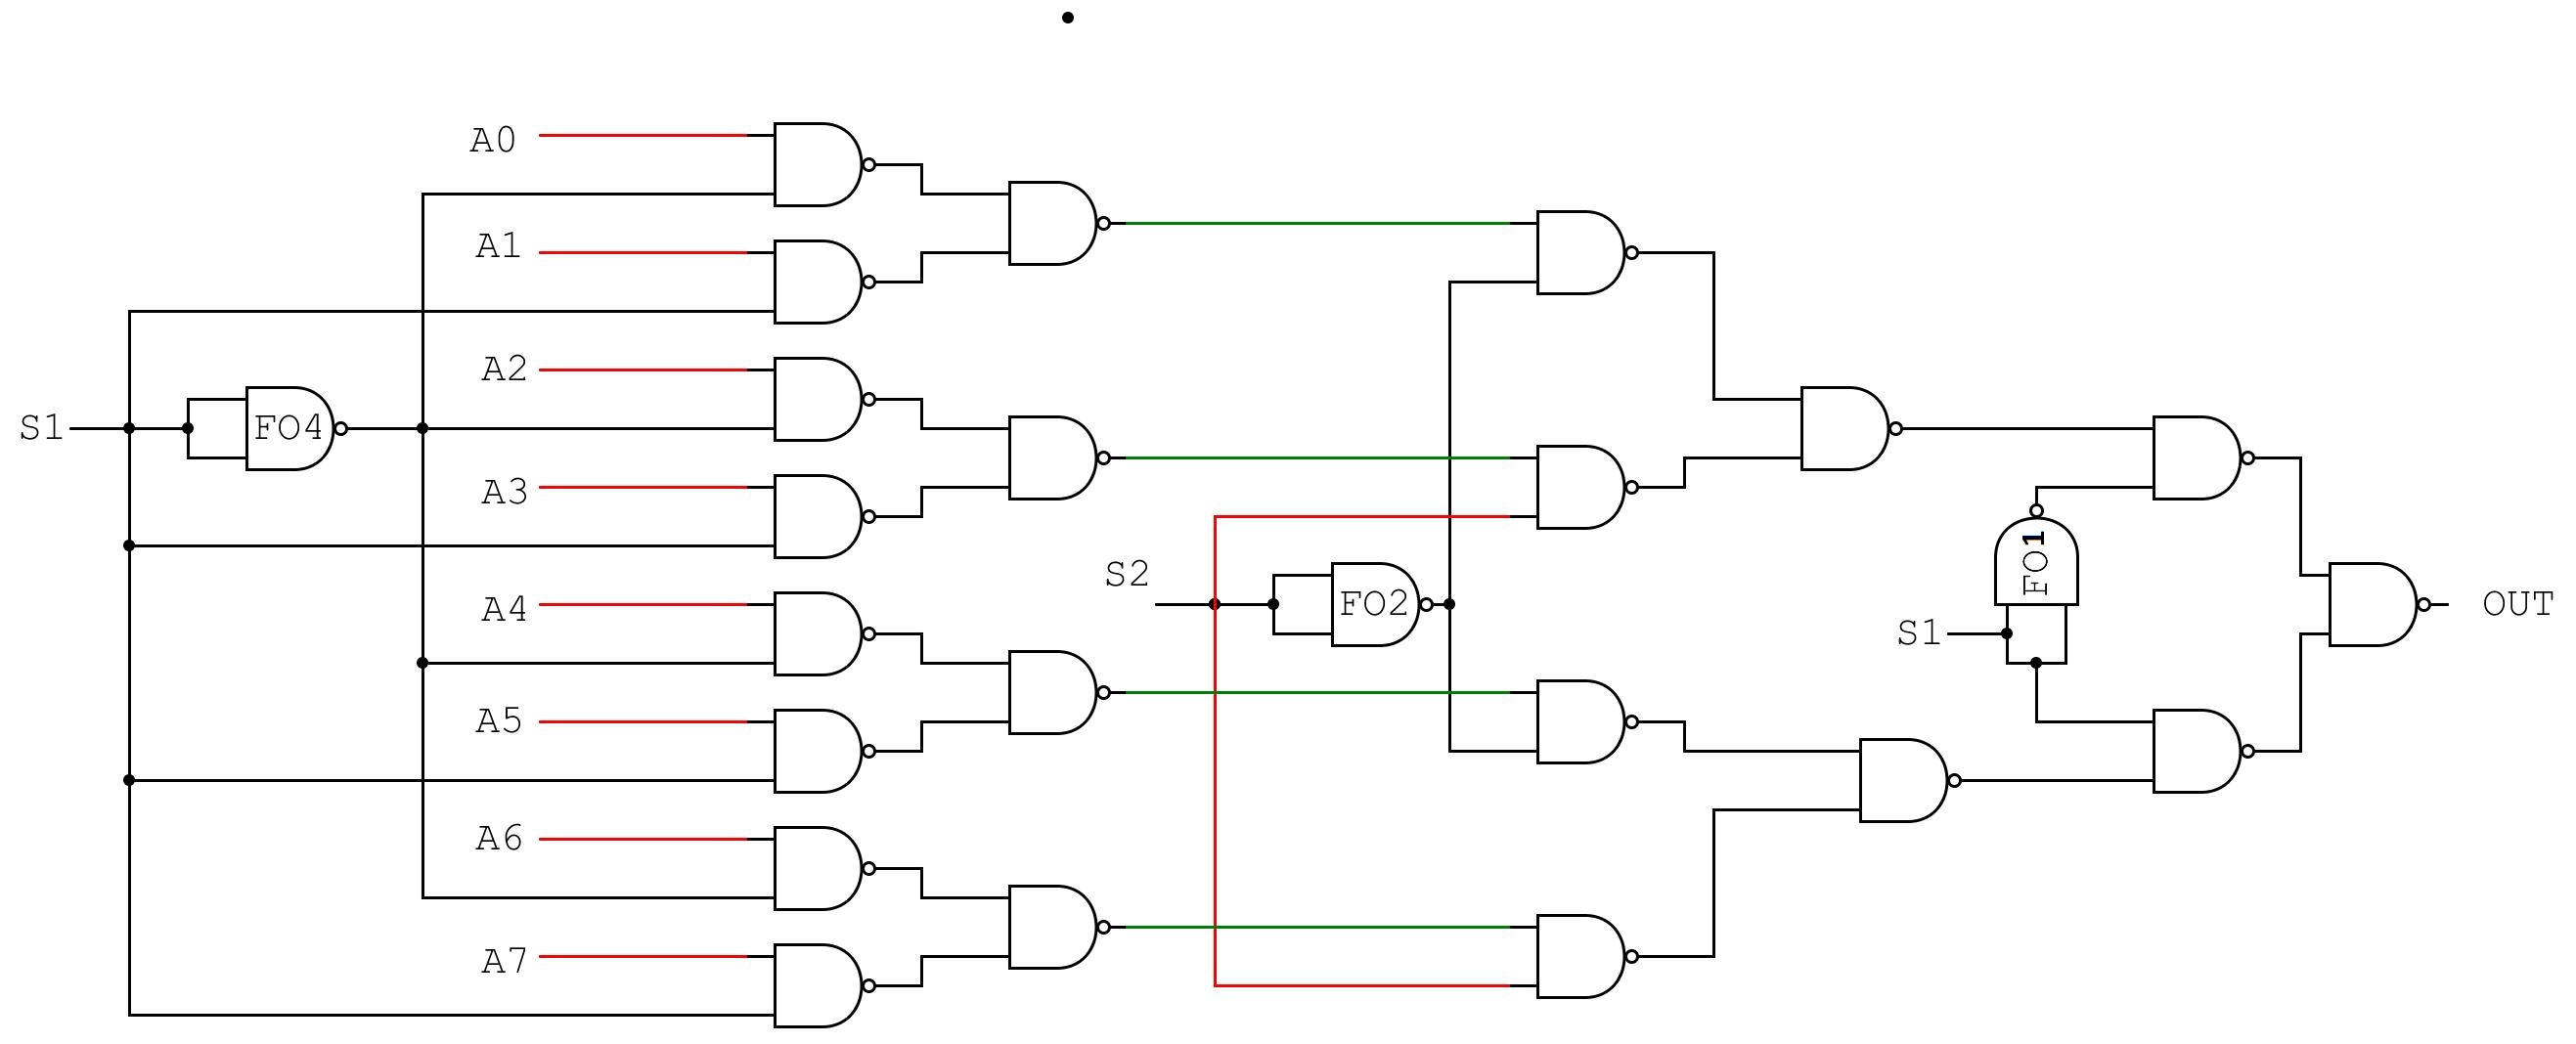
\includegraphics[scale=0.15]{immagini/8_to_1_1bit}
	\caption{\textit{Circuit implementation of a  multiplexer 8 to 1 with only NAND gates.}} 
	\label{8_to_1_1bit}
\end{figure}
\newpage
\section{CMOS realization of multiplexers} 
The next step is to realize a MUX circuit with transistors, by implementing CMOS technology. The building unit is reported in figure \ref{nand2} where a NAND gate is showed.
\begin{figure}[!h]
	\centering
	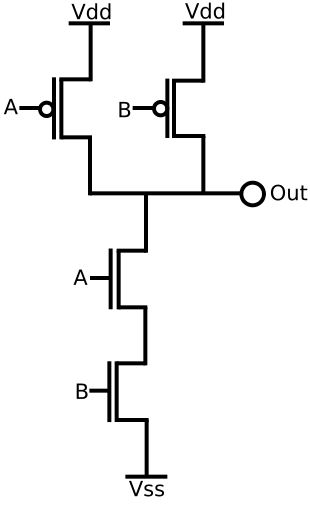
\includegraphics[scale=0.3]{immagini/nand2.png}
	\caption{\textit{CMOS circuit for a NAND gate.}} 
	\label{nand2}
\end{figure}
\newline
An example of CMOS multiplexer realization is reported in the figure below.
\begin{figure}[!]
	\centering
	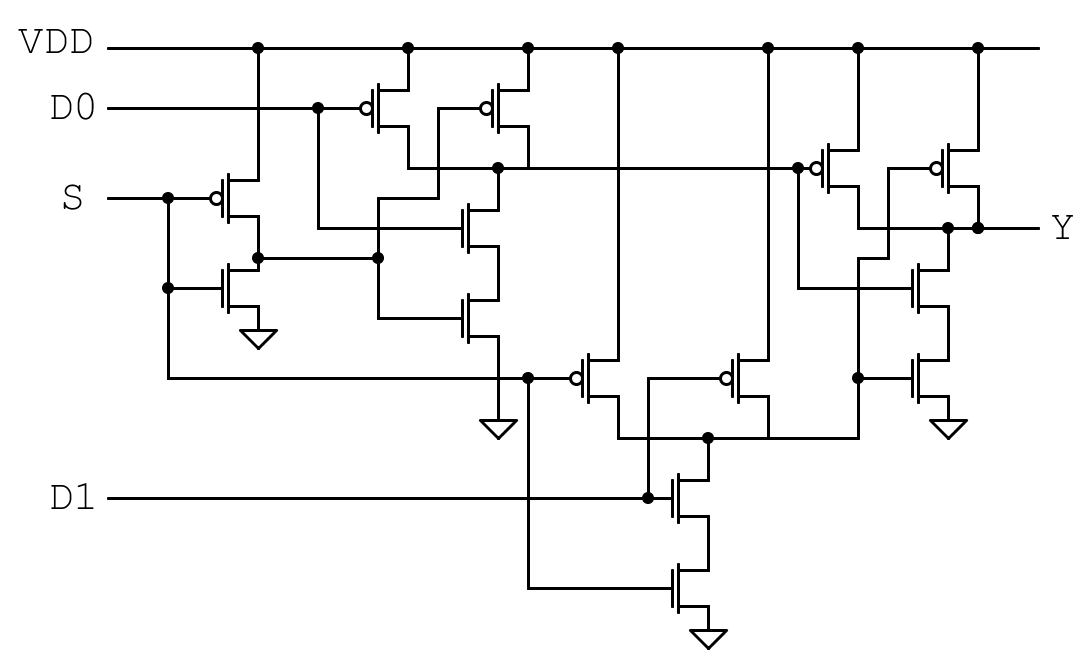
\includegraphics[scale=0.22]{immagini/trans}
	\caption{\textit{CMOS realization of a MUX 2x1.}} 
	\label{mux_3}
\end{figure}

\newpage
\section{Types of Multiplexer}
Here are summarized the different typologies of mutiplexer analysed. The various multiplexers vary by the number of input signals and the parallelism. 
\begin{itemize}\itemsep1pt
	\item Multiplexer 2 to 1 parallelism 16 bit
	\item Multiplexer 2 to 1 parallelism 32 bit
	\item Multiplexer 2 to 1 parallelism 64 bit 
	\item Multiplexer 8 to 1 parallelism 8 bit 	
	\item Multiplexer 16 to 1 parallelism 8 bit
	\item Multiplexer 16 to 1 parallelism 16 bit
	\item Multiplexer 16 to 1 parallelism 32 bit
	\item Multiplexer 16 to 1 parallelism 64 bit 
	\item Multiplexer 32 to 1 parallelism 8 bit
	\item Multiplexer 32 to 1 parallelism 16 bit
	\item Multiplexer 32 to 1 parallelism 32 bit
	\item Multiplexer 32 to 1 parallelism 64 bit 
	\item Multiplexer 64 to 1 parallelism 8 bit
	\item Multiplexer 64 to 1 parallelism 16 bit
	\item Multiplexer 64 to 1 parallelism 32 bit
	\item Multiplexer 64 to 1 parallelism 64 bit 
	\item Multiplexer 128 to 1 parallelism 8 bit
	\item Multiplexer 128 to 1 parallelism 16 bit
	\item Multiplexer 128 to 1 parallelism 32 bit
	\item Multiplexer 128 to 1 parallelism 64 bit 
\end{itemize}
\newpage
\section{NAND with TAMTAMS}
By using the application TAMTAMS web, it was possible to make a first analysis at system level of several parameters concerning CMOS NAND2 gates employed.  The input data used for the analysis are:
\begin{itemize}
	\item Year:\quad 2010;
	\item Technology branch:\quad HP, LOP, LSTP;
	\item model used for $I_{gate}$:\quad Mastar4.
\end{itemize}
From the analysis done we've obtained the following results:
\lstinputlisting{capitoli/code/HP_2010.m}	
%https://tamtams.vlsilab.polito.it/Documentation/TechnologyHTML/bulk/HP2010_dev_bul.html
\lstinputlisting{capitoli/code/LOP_2010.m}	%https://tamtams.vlsilab.polito.it/Documentation/TechnologyHTML/bulk/LOP2010_dev_bul.html
\lstinputlisting{capitoli/code/LSTP_2010.m}	%https://tamtams.vlsilab.polito.it/Documentation/TechnologyHTML/bulk/LSTP2010_dev_bul.html
As can be seen from the previous analysis, different fan out type of NAND2 are available with the respective values of static and dynamic power consumption. This will allow us to built our multiplexers by using different type of gates, reducing the overall occupation area. In particular, to build our multiplexers, we will use NAND gates with fan-out equal to 1, 2 and 4. 

